\clearpage

\section{Misure preliminari}

Come descritto nel paragrafo \ref{cap:Hardware}, sono stati realizzati due differenti sistemi per l'acquisizione di segnali fotopletismografici. L'obiettivo di questo paragrafo è di dimostrarne il funzionamento e i risultati ottenuti. Infatti, occorre verificare che il segnale acquisito sia di buona qualità, affinché il processo successivo di elaborazione porti a stimare i parametri di interesse in modo accurato. Come mostrato nelle figure \ref{fig:foto_moduli_MAX86916} e \ref{fig:foto_moduli_MAXM86161}, sono stati montati, sulle PCB progettate, i sensori PPG, i condensatori e i cavi che permettono l'alimentazione e la comunicazione. Tuttavia, è stato omesso l'accelerometro. Infatti, il seguente lavoro si concentra solamente sulla progettazione e l'acquisizione di segnali in formato grezzo, senza approfondire l'elaborazione degli stessi e gli algoritmi di compensazione dei disturbi causati dai movimenti. Nei seguenti paragrafi, verranno mostrati alcuni risultati ottenuti dalle misurazioni effettuate su due soggetti.

\begin{figure}[bh]
	\centering
	a)
	\includegraphics[width=0.4\linewidth]{ImageFiles/Misure Preliminari/MAX86916}
	b)
	\includegraphics[width=0.4\linewidth]{ImageFiles/Misure Preliminari/MAX86916_euro}
	\caption{a)\textit{Adapter Board} con sensore MAX86916. b)Confronto dimensione dell'\textit{Adapter Board} con una moneta da un euro.}
	\label{fig:foto_moduli_MAX86916}
\end{figure}

\begin{figure}[bh]
	\centering
	a)
	\includegraphics[width=0.4\linewidth]{ImageFiles/Misure Preliminari/MAXM86161}
	b)
	\includegraphics[width=0.4\linewidth]{ImageFiles/Misure Preliminari/MAXM86161_euro}
	\caption{a)\textit{Adapter Board} con sensore MAXM86161. b)Confronto dimensione dell'\textit{Adapter Board} con una moneta da un euro.}
	\label{fig:foto_moduli_MAXM86161}
\end{figure}

\subsection{Segnale PPG}
Il segnale PPG grezzo non rappresenta una stima di un particolare parametro, ma solo grazie ad una successiva elaborazione, tramite opportuni algoritmi, è possibile ottenere informazioni interessanti su alcuni indicatori, come la frequenza cardiaca, la saturazione e la pressione arteriosa.
Tuttavia, osservando la sua morfologia si può valutare la bontà delle acquisizioni\cite{Foroozan2018}. In figura \ref{fig:Descrizione_Segnale_PPG} è mostrato un esempio di segnale PPG ideale. Un segnale fotopletismografico reale è soggetto a del rumore (come sarà ben visibile nel paragrafo \ref{cap:misure_preliminari}, mantenendo le caratteristiche presentate nella figura. Inoltre, esso è un segnale periodico, il cui periodo è definito dal ciclo cardiaco.
\begin{figure}[t]
	\centering
	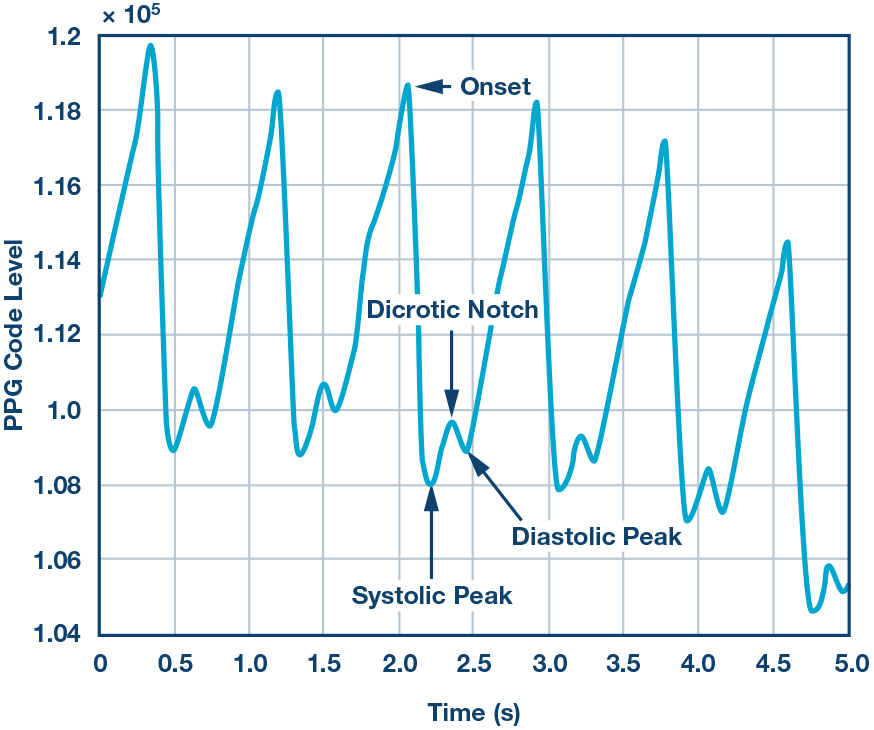
\includegraphics[width=0.7\linewidth]{ImageFiles/Misure Preliminari/descrizione_segnale_ppg}
	\caption{Caratteristiche tipiche di un onda PPG (immagine tratta da Chen\cite{Ppgsignal}).}
	\label{fig:Descrizione_Segnale_PPG}
\end{figure}
`E presente anche una forte similarità tra la morfologia del segnale PPG e la forma d'onda della pressione arteriosa. Infatti, è possibile identificare due picchi separati da un minimo locale (\Fig~\ref{fig:Descrizione_Segnale_PPG}) che corrispondono a dei punti caratteristici della pressione arteriosa: il picco sistolico e il picco diastolico. Essi sono separati da un minimo chiamato tacca dicrotica. La fase sistolica indica la fase di contrazione del muscolo cardiaco, che determina un aumento della pressione all'interno delle arterie, mentre la fase diastolica, compresa tra la tacca dicrotica e il minimo assoluto raggiunto dal segnale prima dell'onda successiva, è indica la fase di rilassamento del cuore\cite{Singh2017}. La tacca dicrotica è tipicamente associata alla chiusura della valvola aortica e determina il termine della fase di sistole\cite{Gamrah2020}.

Il segnale fotopletismografico, una volta acquisito, viene poi elaborato per rimuovere i disturbi. Infatti, esso è molto suscettibile a zone di scarsa perfusione sanguigna, artefatti dovuti al movimento e all'illuminazione dell'ambiente circostante. In alcuni casi, si utilizzano anche altre tipologie di sensori (come ad esempio un accelerometro triassale) per compensare eventuali disturbi.

\subsection{Misurazioni preliminari sui soggetti}\label{cap:misure_preliminari}
Nel seguente paragrafo vengono presentati i risultati ottenuti dalle misurazioni effettuate su due soggetti.
Le misure sono state eseguite seguendo la stessa procedura, in modo da rendere confrontabili, limitando i disturbi causati da differenze nella procedura di acquisizione. Un aspetto importante che è stato osservato sin da subito è l'interazione della luce ambientale sulle misure. Come già ben noto nella letteratura, la luce ambientale introduce delle interferenze che alterano il valore della misura. I disturbi variano da un ambiente all'altro in maniera non prevedibile. Nella figura \ref{fig:ambiente_MAX86916} è rappresentato il segnale acquisito dal sensore PPG MAX86916 lasciandolo esposto alla luce artificiale di una lampadina a LED per uso domestico. Si può notare come il segnale campionato presenti una componente periodica che potrebbe alterare la traccia PPG se il sensore non viene opportunamente isolato.

\begin{figure}[t]
	\centering
	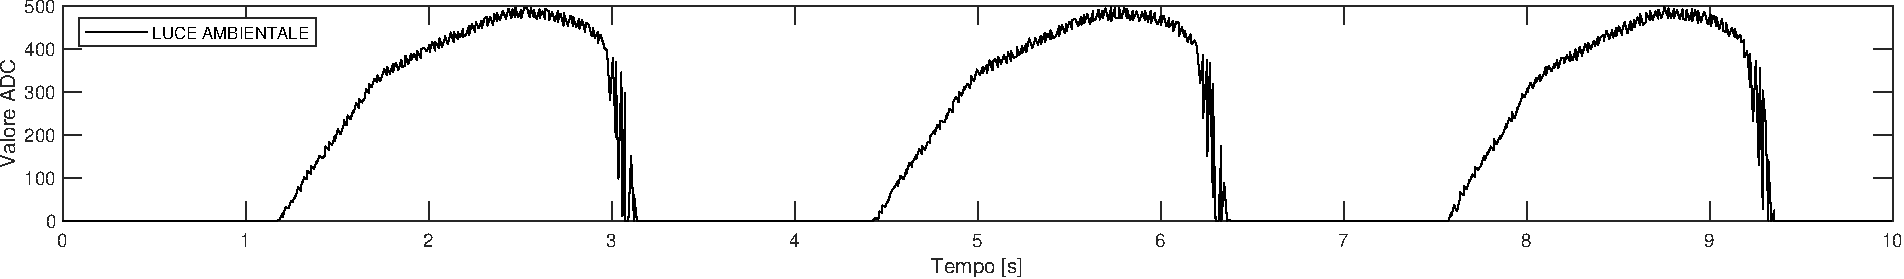
\includegraphics[width=1\linewidth]{ImageFiles/Misure Preliminari/ambiente}
	\caption{Segnale acquisito lasciando il sensore MAX86916 esposto alla luce artificiale.}
	\label{fig:ambiente_MAX86916}
\end{figure}

Per evitare il problema presentato, in questa prima fase del progetto, si è deciso di eseguire tutte le misure in assenza di qualsiasi luce, quindi al buio. In caso non sia possibile un ambiente totalmente al buio è consigliato coprire sensore e il sito di misura con un panno nero, in modo da non permettere alla luce ambientale di penetrare.
Oltre ai disturbi legati alla luce, è necessario anche prevenire gli artefatti dovuti al movimento. Per fare ciò, la soluzione adottata è stata di fissare saldamente l'\textit{Adapter Board} sulla zona idi acquisizione, in modo da evitare spostamenti durante la misura.
Infine, è stato definita la procedura di acquisizione:
\begin{enumerate}
	\item fissare saldamente la board sul sito di misura, in modo che il soggetto sia in posizione stabile e di riposo;
	\item accendere il modulo PPG e attendere 10 secondi, affinché il segnale si stabilizzi;
	\item avviare la registrazione dei campioni per 40 secondi.
\end{enumerate}
Le acquisizioni sono so salvate in un file \textit{csv} tramite il software \textit{SerialPlot}, che interpreta i dati ricevuti dal microcontrollore. Per ogni campione, viene salvato data e ora, espressa in millisecondi, e il valore (espresso in numeri interi \textit{uint\_32}) associato ad ogni canale colore. I dati vengono poi importati nel software \textit{Matlab} per l'analisi.


\paragraph{Configurazione dei moduli PPG}~


\noindent I moduli MAX86916 e MAXM86161, impiegati nelle board progettate, permettono di effettuare diverse configurazioni che dipendono dalla specifica applicazione e dalle caratteristiche che si vogliono ottenere nel segnale acquisito. Di seguito vengono riportate le configurazioni utilizzate per effettuare le misure che verranno successivamente riportate, atte a verificare l'efficacia delle schede realizzate.

\paragraph{Adapater Board: MAXM86161}
Per l'\textit{Adapeter Board} sul quale è montato il sensore MAXM86161 è stata scelta la configurazione riportata in tabella \ref{tab:ConfigMAXM86161}:
\begin{table}[b]
	\renewcommand{\arraystretch}{1.5}
	\centering
	\footnotesize
	\begin{tabular}{cccc}
		\textbf{Numero di campioni mediati} & 1 \\ \hline
		\textbf{Frequenza di acquisizione [Hz]} & 100 \\ \hline
		\textbf{Fondo scala ADC [nA]} & 16384 \\ \hline
		\textbf{Corrente di alimentazione dei LED [mA]} & 9.6 \\ \hline
		\textbf{Tempo di integrazione [$\mu$s]} & 117.3 \\ \hline
		\textbf{Lunghezza impulso [$\mu$s]} & 123.8 \\ \hline
		\textbf{Ritardo di accensione LED [$\mu$s]} & 12 \\ \hline
	\end{tabular}
	\caption{Parametri di configurazione del modulo MAXM86161.}
	\label{tab:ConfigMAXM86161}
\end{table}
La frequenza di campionamento utilizzata è di \SI{100}{\hertz} e non viene eseguita alcuna media \textit{on board} sui campioni acquisiti. In questa fase di test, si è scelto di fornire la medesima corrente a tutti i led. I registri dedicati a definire la sequenza di acquisizione dei led sono stati configurati in modo da accendere in sequenza il led verde, infrarosso e rosso. Ad ogni ciclo di acquisizione viene ripetuta la medesima successione. Il legame tra il tempo di integrazione dell'ADC (t\ped{INT}), il ritardo di accensione dei LED (t\ped{LED\_SETLENGHT}), che permette di attendere che la corrente nel led si stabilizzi e la lunghezza dell'impulso (t\ped{PW}) è mostrato nella figura \ref{fig:tempi_maxm}. In questa fase di test, non sono state attivate le opzioni di risparmio energetico, filtro ALC e \textit{picket fence} in modo da ottenere misure non elaborate.

\begin{figure}[t]
	\centering
	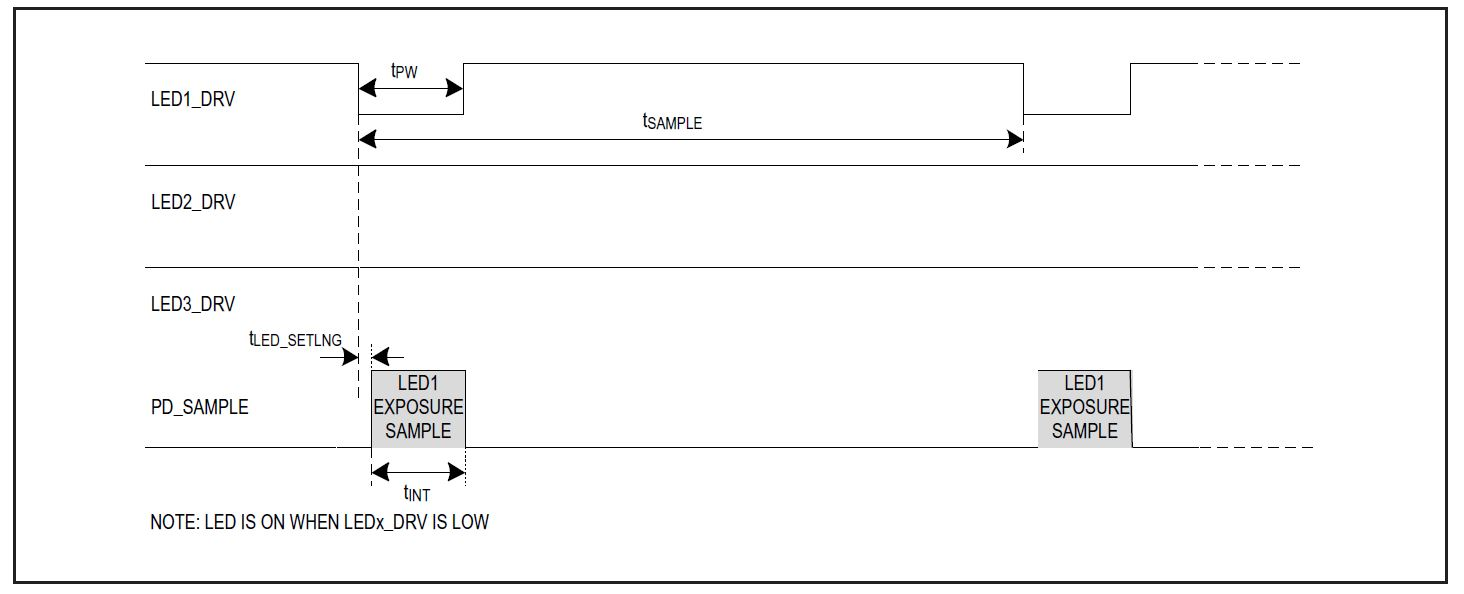
\includegraphics[width=1\linewidth]{ImageFiles/Misure Preliminari/tpower_maxm}
	\caption{Sincronizzazione dei parametri di accensione del led e integrazione dell'ADC con un LED (immagine tratta da Maxim Integrated\cite{IntegratedMAXM86161}).}
	\label{fig:tempi_maxm}
\end{figure}

\paragraph{Adapater Board: MAX86916}
La seconda \textit{Adapeter Board}, con il sensore MAX86916, è stata configurata come riportato in tabella \ref{tab:ConfigMAX86916}:
\begin{table}[b]
	\renewcommand{\arraystretch}{1.5}
	\centering
	\footnotesize
	\begin{tabular}{cccc}
		\textbf{Numero di campioni mediati} & 1 \\ \hline
		\textbf{Frequenza di acquisizione [Hz]} & 100 \\ \hline
		\textbf{Fondo scala ADC [nA]} & 16384 \\ \hline
		\textbf{Corrente di alimentazione dei LED [mA]} & 2.0 \\ \hline
		\textbf{Larghezza impulso luce LED [$\mu$s]} & 420 \\ \hline
		\textbf{Modalità operativa} & FLEX MODE \\ \hline
	\end{tabular}
	\caption{Parametri di configurazione del modulo MAX86916.}
	\label{tab:ConfigMAX86916}
\end{table}
La scelta principale da effettuare è stata quella relativa alla modalità operativa. Dal momento che si vuole verificare il corretto funzionamento della piattaforma, si è deciso di utilizzare la modalità FLEX MODE, dove vengono accesi tutti e quattro i LED del modulo PPG MAX86916. Il valore di corrente fornita è scelto in modo da essere sufficientemente elevato per garantire una buona qualità di segnale, tenendo conto anche della necessità di mantenere bassi valori di corrente per limitare i consumi. L'ADC integrato è stato configurato con un fondo scala di \SI{16384}{\nano\ampere}, che permette di evitare saturazioni in sede di conversione. La frequenza di campionamento scelta invece è di 100Hz e rappresenta una valore intermedio che, in questa fase di studio, è sufficiente per valutare il segnale acquisito. Infine, per la durata dell'impulso della luce emessa dai LED è stato scelto il massimo valore a disposizione, che è di \SI{420}{\micro\second}, in modo da permettere l'assestamento del segnale.

\import{./TextFiles/Progetto della piattaforma indossabile/}{Misure soggetto 1.tex}
\import{./TextFiles/Progetto della piattaforma indossabile/}{Misure soggetto 2.tex}